\documentclass{article}
\usepackage{amsmath}
\usepackage{graphicx}
\usepackage{hyperref}
\usepackage{booktabs}
\title{Age of Astronauts}
\author{Dr. Jamie, You, and Professor X.}
\date{\today}

\begin{document}
\maketitle

\begin{abstract}
This paper presents a statistical analysis of the age trends in astronauts. 
We demonstrate several interesting age-related statistics, as well as showing trends related to space-walk records.
\end{abstract}

\section{Acknowledgements}
This document was drafted with the assistance of Microsoft Copilot.

\section{Introduction}
The age of astronauts has been a topic of interest for many years. 
This paper presents a statistical analysis of the age of astronauts and some related analysis around age and spacewalk records.

\section{Methodology}
The data for this study was collected from the Tidy Tuesday data repository \cite{tidytuesday}, entry 2020-07-14, and analyzed using Python with the pandas \cite{reback2020pandas,mckinney-proc-scipy-2010} package.

\section{Results}
The results of the analysis show the average age of astronauts at their selection and mission.

\begin{table}[h]
\centering
\begin{tabular}{lrr}
\toprule
 & Age on selection & Age on mission \\
\midrule
min & 24.000000 & 28.000000 \\
max & 60.000000 & 77.000000 \\
median & 34.000000 & 43.000000 \\
mean & 34.158127 & 43.496466 \\
\bottomrule
\end{tabular}

\caption{Age of astronauts at selection and mission.}
\label{tab:sample_table}
\end{table}

We additionally explore how the record spacewalk length has changed over time in Figure \ref{fig:spacewalkrecord}, as well as how this is related to the age of astronauts. 

\begin{figure}[h]
\centering
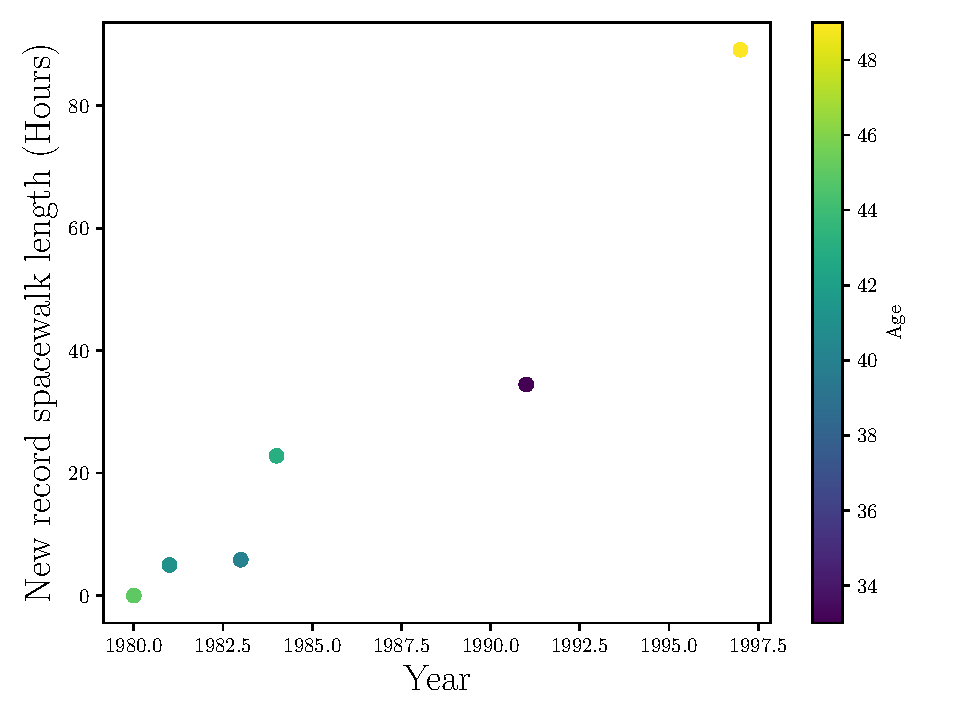
\includegraphics[width=\textwidth]{../analysis/spacewalk_record.pdf}
\caption{Spacewalk record over time, as well as the age of the astronaut setting the record at the time of the mission.}
\label{fig:spacewalkrecord}
\end{figure}

\section{Discussion}
The average age of astronauts could be attributed to several factors. 
Changes in the selection criteria for astronauts may affect the average age over time. 
This analysis will be considered in future work.

\bibliographystyle{plain}
\bibliography{refs}

\end{document}